\icode{E-MD-CA-L3-261112-008}
如图所示，将木块 \(A\) 和木板 \(B\) 叠放在水平地面上，木块质量 \(m_A =\) \,\qty{2}{kg}，木板质量 \(m_B =\)\qty{1}{kg}，木块与木板间动摩擦因数为 \(\mu_1 = 0.3\)、木板与地面间动摩擦因数为 \(\mu_2 = 0.1\)，不计空气阻力，取重力加速度 \(g =\) \,\qty{10}{m/s^2}，设最大静摩擦力等于滑动摩擦力，对木块施加一个水平向右的恒力 \(F\)，求：
\begin{enumerate}
	\item 若 \(F =\) \,\qty{9}{N}求木块 \(A\) 的加速度大小和 \(A\)、\(B\) 之间的摩擦力的大小；
	\item 若 \(F =\) \,\qty{16}{N}，求木块 \(A\) 的加速度大小和 \(A\)、\(B\) 之间的摩擦力的大小。
\end{enumerate}

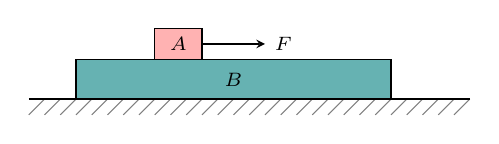
\begin{tikzpicture}[>=stealth,font=\scriptsize]
	\draw[fill=teal!60] (0,0) rectangle(4,.5)node[midway]{\(B\)};
	\draw[fill=red!30] (1,.5) rectangle(1.6,.9)node[midway]{\(A\)};
	\draw[->] (1.6,.7)--++(.8,0)node[right]{\(F\)};
	\foreach \x in {-.6,-.4,...,5}
		\draw[gray] (\x,-.2)--++(.2,.2);
	\draw[thick] (-.6,0)--(5,0);
\end{tikzpicture}
\begin{answer}
    
\end{answer}